\documentclass[aspectratio=169,10pt]{beamer}
\usetheme{default}
\usepackage[T1]{fontenc}
\usepackage[utf8]{inputenc}
\usepackage{lmodern}
\usepackage{booktabs}
\usepackage{graphicx}

\definecolor{ink}{HTML}{0B0B0B}
\definecolor{muted}{HTML}{52514E}
\definecolor{treecol}{HTML}{2A78D6}
\definecolor{lrcol}{HTML}{EB6834}
\definecolor{ebmcol}{HTML}{1BAF7A}
\setbeamercolor{frametitle}{fg=ink}
\setbeamercolor{normal text}{fg=ink}
\setbeamercolor{itemize item}{fg=muted}
\setbeamerfont{frametitle}{size=\large,series=\bfseries}
\setbeamertemplate{navigation symbols}{}
\setbeamertemplate{itemize items}[circle]
\setbeamertemplate{footline}{%
  \hspace{1em}\textcolor{muted}{\tiny Explainable Classification of Payment Difficulty --- T.\,S.\,A. Camargo, J. Corrales Almendariz, J. Montes de Oca Martínez --- IAE, UPM, October 2026}%
  \hfill\textcolor{muted}{\tiny\insertframenumber/4}\hspace{1em}\vspace{0.6em}}
\graphicspath{{../report/figures/}}
\newcommand{\sw}[1]{\textcolor{#1}{$\blacksquare$}}

\begin{document}

% ---------------------------------------------------------------------------
\begin{frame}{What we did and what we found}
\begin{columns}[T]
\begin{column}{0.47\textwidth}
\small
\vspace{-0.6em}
\textbf{Task.} Predict next-month payment difficulty (21\,\% positives; 25k labelled clients, 15 predictors).

\textbf{Protocol.} 80/20 training/validation split. \emph{Every} choice (hyperparameters, log transform, threshold) is made with the \emph{same} 5 CV folds; the validation set is used once for confirmation.
\begin{itemize}\setlength\itemsep{0pt}
\item Tuning by CV AUC; one-SE rule $\Rightarrow$ simplest model
\item No class weights: CV-chosen thresholds $t_{\text{acc}}\approx0.5$ (submission), $t_{\text{bal}}\approx0.2$ (analysis)
\item Common yardsticks: permutation importance, log-odds effect curves, additive local decompositions
\end{itemize}

\textbf{Findings.} EBM best in 5/5 folds, and better than a black box. Same drivers in all models, but different \emph{carriers} and \emph{shapes} $\Rightarrow$ local conflicts. \textbf{Submitted: EBM.}
\end{column}
\begin{column}{0.51\textwidth}
\footnotesize
\begin{tabular}{@{}lccc@{}}
\toprule
5-fold CV & AUC & Acc. & Bal.\ acc. \\
\midrule
\sw{treecol} Tree (17 leaves) & .752 & .812 & .692 \\
\sw{lrcol} Logistic regression & .761 & .814 & .695 \\
\sw{ebmcol} EBM (\texttt{interactions=0}) & \textbf{.776} & \textbf{.817} & \textbf{.705} \\
\midrule
Majority baseline & .500 & .788 & .500 \\
Black box (HistGB) & .768 & .815 & .701 \\
\bottomrule
\end{tabular}

\vspace{0.4em}
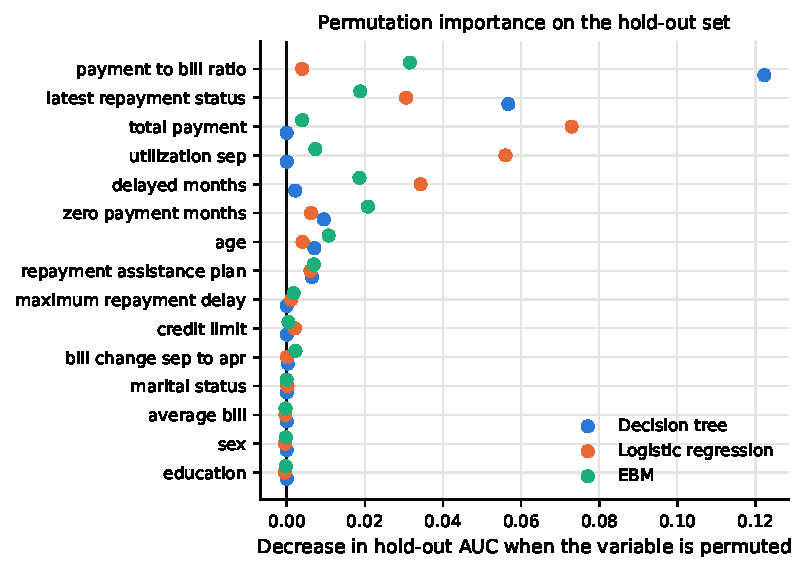
\includegraphics[width=\linewidth]{permutation_importance.pdf}
\end{column}
\end{columns}
\end{frame}

% ---------------------------------------------------------------------------
\begin{frame}{\sw{treecol}\ Decision tree: 17 leaves collapse into a 6-rule risk profile}
\begin{columns}[T]
\begin{column}{0.5\textwidth}
\footnotesize
\textbf{Flag difficulty if any rule fires} (status = latest repayment status, ratio = payment-to-bill ratio):

\vspace{0.3em}
\begin{tabular}{@{}lp{0.68\linewidth}c@{}}
\toprule
 & Rule & Risk \\
\midrule
R1 & status $\geq1$ and ratio $\leq0.095$ & .54 \\
R2 & status $\leq0$ and ratio $\leq0.025$ & .43 \\
R3 & status $\geq1$, ratio $>0.095$, zero-pay months $\geq4$ & .33 \\
R4 & status $\leq0$, ratio $\in(0.025,0.105]$, age $\leq24$ & .32 \\
R5 & status $\geq1$, ratio $\in(0.095,0.315]$, zero-pay $\leq3$ & .28 \\
R6 & status $\leq0$, ratio $\in(0.025,0.105]$, age $\geq25$, plan & .26 \\
\bottomrule
\end{tabular}

\vspace{0.4em}
\begin{itemize}\setlength\itemsep{0pt}
\item R1 alone: 15\,\% of clients, 39\,\% of all difficulties
\item Uses only 7 of 15 variables; 85\,\% of the impurity reduction comes from status and ratio
\item Most \emph{simulatable} model, but the coarsest (17 probability levels)
\end{itemize}
\end{column}
\begin{column}{0.48\textwidth}
\footnotesize
\textbf{Local case C} (actual: difficulty): 1 month late, 4/6 months delayed, plan, \emph{negative bill} $\Rightarrow$ ratio 4.39.

\vspace{0.2em}
Tree path: status $\geq1$ $\to$ ratio $>0.095$ $\to$ treated as \emph{protective} ($-1.25$ log-odds) $\Rightarrow$ $p=0.15$, \textbf{missed}.

\vspace{0.2em}
LR ($p=0.50$) and EBM ($p=0.55$) read the high ratio as \emph{risk} and add the delayed months $\Rightarrow$ correctly flagged.

\vspace{0.3em}
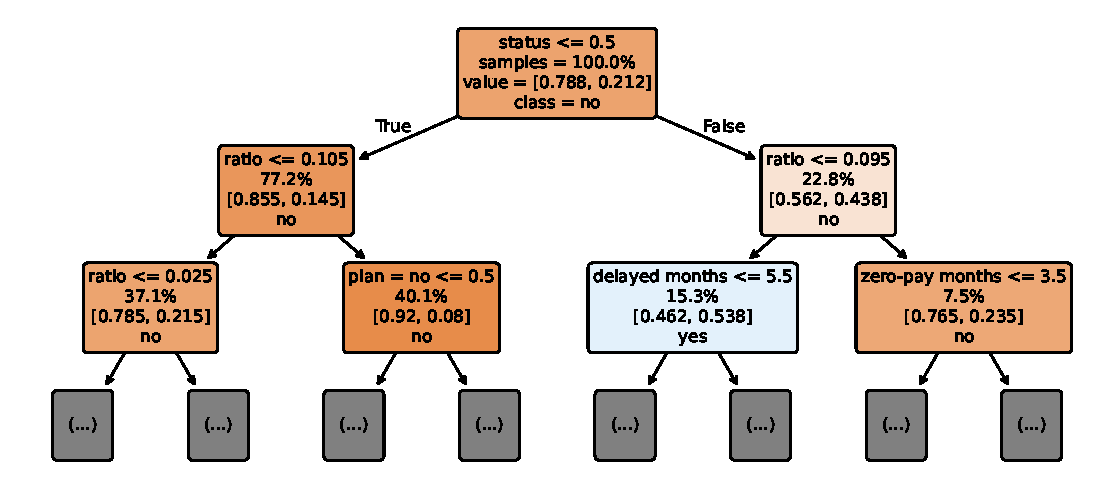
\includegraphics[width=\linewidth,trim=0 0 0 0,clip]{tree_top_levels.pdf}
\end{column}
\end{columns}
\end{frame}

% ---------------------------------------------------------------------------
\begin{frame}{\sw{lrcol}\ Logistic regression: compact, stable, but conditional and linear}
\begin{columns}[T]
\begin{column}{0.46\textwidth}
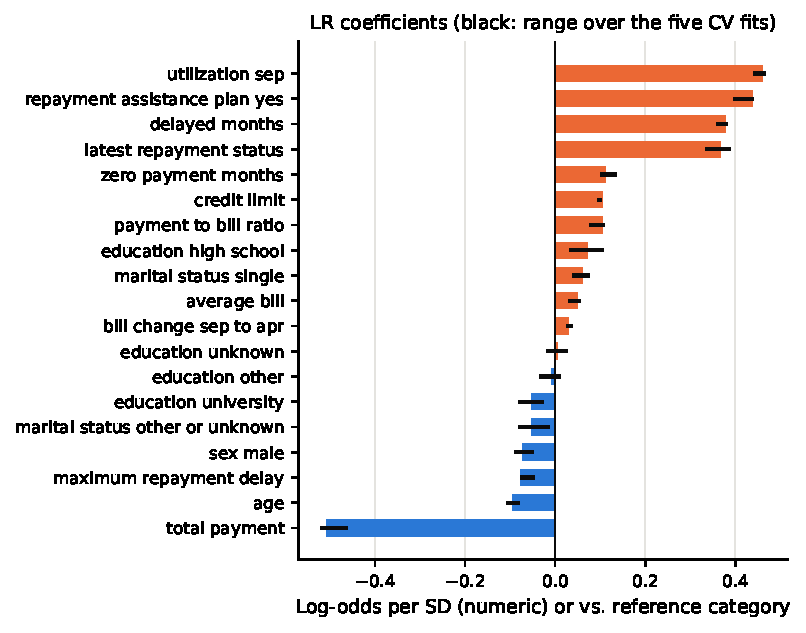
\includegraphics[width=\linewidth]{logit_coefficients.pdf}
\end{column}
\begin{column}{0.52\textwidth}
\small
\begin{itemize}\setlength\itemsep{2pt}
\item Standardized inputs, reference coding; a CV-selected signed-log transform of money variables raises AUC from .750 to .762
\item Strongest effects: utilization $+0.46$/SD, assistance plan $+0.44$ (OR 1.55), delayed months $+0.38$, status $+0.37$, log total payment $-0.51$
\item Signs stable over the 5 CV refits, \textbf{but conditional}: max.\ delay ($r=+.27$ with the target, $\beta=-.08$), credit limit and payment ratio all \emph{reverse} their marginal sign because of collinearity
\item Linear in the undocumented status codes $-2,-1,0$
\end{itemize}
\footnotesize
\textbf{Local case D} (actual: no difficulty): up to date on everything, but utilization 2.0 $\Rightarrow$ $+1.80$ log-odds, $p=0.39$, \textbf{false alarm} (EBM $0.28$ also). The tree ignores utilization: $p=0.06$, correct.
\end{column}
\end{columns}
\end{frame}

% ---------------------------------------------------------------------------
\begin{frame}{\sw{ebmcol}\ EBM: the shapes behind the best model}
\centering
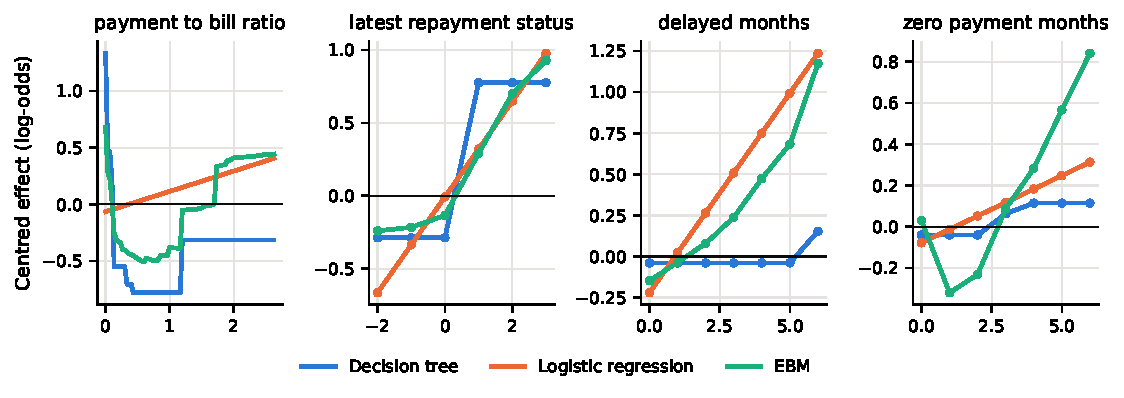
\includegraphics[width=0.86\linewidth]{effect_comparison.pdf}

\vspace{-0.3em}
\begin{columns}[T]
\begin{column}{0.49\textwidth}
\footnotesize
\begin{itemize}\setlength\itemsep{1pt}
\item \textbf{Payment ratio is U-shaped}: risk is lowest at 0.5--1.2 and rises again above 1.7 (catch-up payments, tiny bills). The tree is flat there; LR can only fit a straight line.
\item \textbf{Zero-payment months}: 1--2 are protective, 3+ are harmful; \textbf{age} is U-shaped (under 25, over 57).
\item Assistance plan $+0.41$: a marker of prior stress, \emph{not} a causal harm.
\end{itemize}
\end{column}
\begin{column}{0.49\textwidth}
\footnotesize
\begin{itemize}\setlength\itemsep{1pt}
\item Permutation-importance rank correlation: tree--EBM .85, LR--EBM .73, tree--LR .36. This is the \emph{Rashomon effect} on redundant payment variables.
\item Local explanations are exact sums of the shapes. Case B (all correct): status~2 and the plan dominate in all three models.
\end{itemize}
\end{column}
\end{columns}
\end{frame}

\end{document}
